\section{Instrumenting Microservices} \label{sec:impl}
In this section, we explain the implementation of the instrumentation algorithm for microservices-based applications, as well as a demo of how the tool modifies these applications based on different logging specifications. In our instrumentation tool, each microservice of an application is treated as an agent of the concurrent system, whereas each method defined in some library of a microservice is considered as a sub-agent.% of that agent.

\subsection{Instrumentation Tool: $\tool$} \label{sec:impl-tool}
We have implemented the proposed algorithm $\rewrite$ for microservices-based applications that are deployed using Java Spring Framework. % \cite{johnson2004spring}. 
Our instrumentation tool \cite{github1}, 
$\tool$, receives a logging specification along with an application consisting of two or more microservices, and rewrites those microservices accordingly. $\tool$ extends microservices with required RESTful APIs that facilitate the communication between microservices for the sake of audit logging. %$\tool$ receives three arguments described in the following.

The logical specification of logging requirements (Section \ref{sec:logspec}) is passed as an argument to $\tool$ in JSON format. $\tool$ parses this JSON file and extracts logging specification in the form of Horn clauses, along with identifying triggers and logging events.
The paths to different microservices of the application are also passed to $\tool$. %For this purpose, $\tool$ expects a file with paths to different microservices. These microservices are supposed to be built by Java Spring Framework. 
$\tool$ applies modifications to each microservice component according to the logging specification.
In addtion, the path to the Prolog engine must be fed to $\tool$. $\tool$ uses SWI Prolog \cite{swi} to logically infer the derivation of logging events according to the logging specification, the set of facts regarding trigger events, etc.% as well as any other collection of facts that are potentially needed\footnote{Note that there could be preconditions beyond trigger events.}.

%\begin{itemize}
%	\item The logical specification of logging requirements (Section \ref{sec:logspec}) is passed as an argument to $\tool$ in JSON format. $\tool$ parses this JSON file and extracts logging specification in the form of Horn clauses, along with identifying triggers and logging events.
%	\item The microservices-based application is passed as another argument to $\tool$. For this purpose, $\tool$ receives a text file with paths to different microservices. These microservices are supposed to be built by Java Spring Framework. $\tool$ applies modifications to each microservice component according to the logging specification.
%	\item The last argument to $\tool$ is the path to the Prolog engine in the local system. $\tool$ uses SWI Prolog \cite{swi} to logically infer the derivation of logging events according to the logging specification, the set of facts regarding trigger events, as well as any other collection of facts that are potentially needed\footnote{Note that there could be arbitrary preconditions in the logging specification that may require gathering facts beyond trigger events.}.
%\end{itemize}

$\tool$ uses aspect-oriented programming (AOP), in particular AspectJ, %\cite{laddad2009aspectj}, 
to weave concurrent logging capability into microservices. For this purpose, $\tool$ extends the Project Object Model of the microservices which need to be instrumented by \texttt{spring-boot-starter-aop} dependency. 
%(Figure \ref{fig:aop-dep}).
%
%\begin{figure}
%\begin{scriptsize}
%\begin{Verbatim}[frame=single]
%...
%<dependency>
%  <groupId>org.springframework.boot</groupId>
%  <artifactId>spring-boot-starter-aop</artifactId>
%</dependency>
%...
%\end{Verbatim}
%\end{scriptsize}
%\caption{AOP dependency.}
%\label{fig:aop-dep}
%\end{figure}

According to the implementation model, the configuration of the concurrent system includes three different structures to store the logging preconditions that are transpired locally ($\locprec$), logging preconditions that are originated remotely ($\remprec$), and the audit logs recorded by an agent ($\logmap$). These structures are added by $\tool$ as repositories of logical facts that are kept on nonvolatile memory. If a microservice is only a trigger, then a repository is added to that microservice to store logging preconditions that take place locally in that microservice. However, if a microservice is a logging event, then that microservices is extended with all three types of repositories. 
%to store locally and remotely transpired preconditions, as well as the audit logs. 
We call these repositories \texttt{local-db}, \texttt{remote-db}, and \texttt{log-db}, resp. Note that according to the definition of $\rewrite$ (Section \ref{sec:inst-alg}), a trigger is only concerned with locally transpired preconditions (through $\callev$ prefixes), whereas a logging event needs to access all three types of aforementioned structures (through $\callev$, $\addprecond$, and $\emitev$ prefixes).

$\rewrite$ extends every trigger with sub-agents, $D_{ij}$, that send back the locally generated preconditions upon receiving a request on a dedicated link (using $\sendprecond$ prefix). $\tool$ implements this feature by extending each trigger microservice with a REST controller that sends back the content of \texttt{local-db}, if it receives an HTTP GET request on the dedicated path \texttt{/localdb}. This controller is denoted by \texttt{LocalDBController}, henceforth. On the other side, a logging event microservice is supposed to contact the trigger on dedicated links to receive the preconditions that are transpired in trigger agents. $\tool$ facilitates this by extending every logging event microservice with a web client that sends asynchronous HTTP GET requests to \texttt{/localdb} path on trigger microservices and collects the responses. We have called this service \texttt{RestClient}.

As mentioned earlier, AOP is used to add logging capabilities to microservices. For this purpose, $\tool$ identifies the pointcuts in which an advice needs to be defined. According to $\rewrite$, trigger sub-agents are preceded by $\callev$ prefixes. For this purpose, $\tool$ defines \textit{before} aspects for each of the trigger methods, where the advice includes the construction of preconditions from the join points and adding them to \texttt{local-db}. This implements the semantics of $\callev$.%, given in Figure \ref{fig:before-asp}.

$\rewrite$ instruments logging event sub-agents by inserting a sequence of operations before the execution of these sub-agents. This sequence includes $\callev$ prefixes, communication on dedicated links to receive remotely transpired logging preconditions, adding them to $\remprec$ using $\addprecond$ prefixes, and finally checking if logging events should to be logged, using $\emitev$. $\tool$ handles this by defining \textit{before} aspects for the pointcuts that correspond to logging event methods. Similar to the aspects defined for trigger methods, the advice for logging event methods starts with the construction of preconditions from join points and adding them to \texttt{local-db}. Next, \texttt{RestClient} is used to asynchronously send an HTTP GET request on the predefined path \texttt{/localdb} to each of the trigger microservices, and collect the results in \texttt{remote-db}. This implements the semantics of $\addprecond$ prefix. Then, SWI Prolog engine is invoked to add the logging specification, and the contents of \texttt{local-db} and \texttt{remote-db}. Finally, the Prolog engine is queried to study if the invocation of logging event must be logged, and accordingly \texttt{log-db} repository is updated. These final steps implement the semantics of $\emitev$ prefix. In order to facilitate the communication between SWI Prolog engine and Java Virtual Machine, InterProlog Java/Prolog SDK \cite{calejo2004interprolog} is used. 

Figure \ref{fig:before-asp} specifies the advice for triggers and logging events in general form. Figure \ref{fig:log-inst} depicts some of the aforementioned modifications that $\tool$ applies architecturally to the logging event and trigger microservices.

\begin{figure}
\begin{tiny}
\begin{Verbatim}[frame=single]
@Before("execution (some trigger)")
public void someAspect(JoinPoint){
	...
	build precondition from JoinPoint
	add precondition to local-db
	...
}

@Before("execution (some logging event)")
public void someAspect(JoinPoint) {
	...
	build precondition from JoinPoint
	add precondition to local-db
	...
	send GET to triggers
	collect the responses in remote-db
	...
	add logging specification to the engine
	add the content of local-db to the engine
	add the content of remote-db to the engine
	query the engine and update log-db
	...	
}
\end{Verbatim}
\end{tiny}
\caption{Pseudocode of \textit{before} advice for triggers and logging events.}
\label{fig:before-asp}
\end{figure}


%\begin{figure}
%\begin{scriptsize}
%\begin{Verbatim}[frame=single]
%
%\end{Verbatim}
%\end{scriptsize}
%\caption{Pseudocode of \textit{before} advice for logging events.}
%\label{fig:before-asp-logev}
%\end{figure}


%\subsection{A Demo of Microservices-based Medical Records Systems} \label{sec:impl-demo}
\subsection{Case Study: Instrumenting $\demo$ with $\tool$} \label{sec:cstudy}
In Section \ref{sec:intro}, we discussed an oversimplified MRS consisting of several loosely-coupled microservices. We have implemented \cite{github2} 
a demo of this system, $\demo$, consisting of several microservices, using Java Spring Boot \cite{webb2013spring}. The front-end microservice of $\demo$ authenticates users and acts as the API gateway by relaying requests to the back-end microservices. %$\demo$ consists of the following microservices.

%\paragraph{\texttt{authorization-service}} 
%\textbf{\texttt{authorization-service.}}
%This microservice provides different functionalities regarding user access to system resources. The main component of this microservice is a REST controller that provides API to check access status of some user to a system resource, break the glass by some user, check if the glass is broken for some user, and retrieve the list of users who have currently broken the glass.

%\paragraph{\texttt{patient-service}} 
%\textbf{\texttt{patient-service.}}
%This microservice implements patient data model, which includes patient ID, name, and patient disease. Patient microservice uses Java Persistent API (JPA) to map patient data model to a relational database entity. It includes an extension to JPA repository interface that manages access to the patient entity. Patient microservice uses a relational database for this purpose. %\cite{h2db} swhich is populated by a SQL file from disk at the startup.
%\footnote{Indeed, in a more realistic setting, a database management system with nonvolatile storage must be used.}. 
%Patient microservice includes a REST controller that provides API to read patient information from the database using JPA repository interface. The API includes retrieving 1) patient medical history by ID and patient name, 2) all patients with a certain disease, and 3) the information of all patients.


%\begin{figure} [h]
%	\centering
%	\fbox{
\includegraphics[width=0.45\textwidth]{./figs/log-inst.eps}}
%	\caption{Structure of the logging event and trigger microservices, instrumented by $\tool$.}
%	\label{fig:log-inst}
%\end{figure}

%\paragraph{\texttt{authentication-service}} 
%\textbf{\texttt{authentication-service.}}
%This microservice implements the application front-end as a web user interface through a collection of Java Server Pages, as well as two proxies that provide APIs to communicate with the two other microservices. The application front-end uses a login service that mimics the authentication of users based on their credentials. Authentication microservice defines REST controllers that employ OpenFeign proxies to relay user requests (coming from web UI) to Patient and Authorization microservices.

%\begin{itemize}
%	\item Authorization Microservice (\texttt{authorization-service}): This microservice provides different functionalities regarding user access to system resources. The main component of this microservice is a REST controller that provides API to check access status of some user to a system resource, break the glass by some user, check if the glass is broken for some user, and retrieve the list of users who have currently broken the glass.
%%	\begin{itemize}
%%		\item check access status of some user to a system resource,
%%		\item break the glass by some user,
%%		%\item mend the glass by some user,
%%		\item check if the glass is broken for some user, and
%%		\item retrieve the list of users who have currently broken the glass.
%%	\end{itemize}
%	
%	\item Patient Microservice (\texttt{patient-service}): This microservice implements patient data model, which includes patient ID, name, and patient disease. Patient microservice uses Java Persistent API (JPA) to map patient data model to a relational database entity. It includes an extension to JPA repository interface that manages access to the patient entity. Patient microservice uses H2 in-memory database \cite{h2db} which is populated by a SQL file from disk at the startup\footnote{Indeed, in a more realistic setting, a database management system with nonvolatile storage must be used.}. Patient microsevice includes a REST controller that provides API to read patient information from H2 database using JPA repository interface. The API includes retrieving patient medical history by ID, retrieving patient medical history by name, retrieving all patients with a certain disease, and retrieving the information of all patients.
%%	\begin{itemize}
%%		\item retrieving patient medical history by ID,
%%		\item retrieving patient medical history by name,
%%		\item retrieving all patients with a certain disease, and
%%		\item retrieving the information of all patients.
%%	\end{itemize}
%	
%	\item Authentication Microservice (\texttt{authentication-service}): This microservice implements the application front-end as a web user interface through a collection of Java Server Pages, as well as two Feign proxies that provide APIs to communicate with the Authorization and Patient microservices. The application front-end uses a login service that mimics the authentication of users based on their credentials. Authentication microservice defines REST controllers that employ OpenFeign proxies to relay user requests (coming from web UI) to Patient and Authorization microservices.
%\end{itemize}
%Figure \ref{fig:mrs-mics-impl} demonstrates the high-level architecture $\demo$.

%Figure \ref{fig:mrs-mics} depicts the high-level structure of $\demo$, where the application front-end is the Authentication microservice.

%\begin{figure} 
%	\centering
%	\fbox{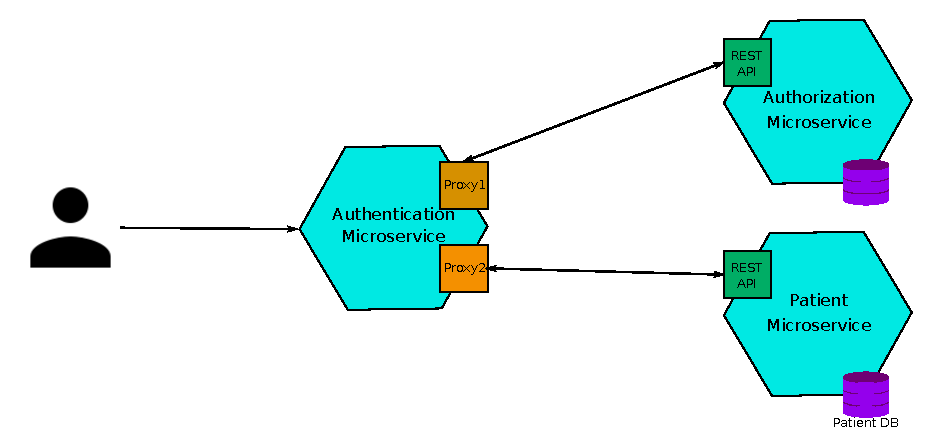
\includegraphics[width=0.45\textwidth]{./figs/mrs-mics3.eps}}
%	\caption{High-level architecture of $\demo$.}
%	\label{fig:mrs-mics-impl}
%\end{figure}

%\subsection{Case Study: Instrumenting $\demo$ with $\tool$} \label{sec:cstudy}
%As mentioned in Section \ref{sec:impl-tool}, $\tool$ receives the logging specification in JSON format, along with the different microservices of a system that may need to be instrumented. As a case study, 
In the following, we explain how $\demo$ is instrumented by $\tool$ for a given logging specification. In Figure \ref{fig:exm-logspec}, we have described a logging specification that enforces logging access to patient medical history at any point after breaking the glass. We can assert a similar logging specification rule in JSON \cite{github1}
, which is more verbose than its logical equivalent. $\tool$ parses that JSON specification and constructs the Horn clause given in Figure \ref{fig:brk-horn} (ver. 1), which is then added to SWI Prolog engine fact base.
Note that in this Horn clause presentation, we have redacted the full package names of the trigger and logging event methods and replaced them with \texttt{<package>}, for the sake of space economy.  $\tool$ instruments $\demo$ according to this logging specification rule as follows: \texttt{spring-boot-starter-aop} dependency is added to the POM of Patient and Authorization services. Authorization service is extended with  \texttt{local-db}.  Patient service is extended with \texttt{local-db}, as well as \texttt{remote-db}, and \texttt{log-db}. Authorization service is extended with the REST controller \texttt{LocalDBController} that responds to requests on path \texttt{/localdb}.  Patient service is extended with \texttt{RestClient} web client. A \textit{before} aspect is added to Authorization service with \texttt{AuthorizationController.breakTheGlass} as its pointcut. This aspect builds preconditions from the join point and appends them to \texttt{local-db}. A \textit{before} aspect is added to Patient service with pointcut \texttt{PatientController.getPatientMedHistByName}, to 1) build preconditions from the join point and append them to \texttt{local-db}, 2) send HTTP GET request on path \texttt{/localdb} to Authorization service, and store the results in \texttt{remote-db} repository,  3) add the logging specification, and contents of \texttt{local-db} and \texttt{remote-db} repositories to the SWI Prolog engine, and 4) send queries to the Prolog engine to check derivability of \texttt{loggedfunccall} predicates and accordingly update \texttt{log-db} with the engine's response.
 
%1) \texttt{spring-boot-starter-aop} is added as a dependency to the POM of both \texttt{patient-service} and \texttt{authorization-service}. 2) \texttt{local-db} repository is added to  \texttt{authorization-service}. 3) \texttt{local-db}, \texttt{remote-db}, and \texttt{log-db} repositories are added to \texttt{patient-service}. 4) \texttt{LocalDBController} is added to  \texttt{authorization-service} to respond to requests on path \texttt{/localdb}. 5) \texttt{patient-service} is extended with \texttt{RestClient} web client service. 6) A \textit{before} aspect is added to \texttt{authorization-service} with \texttt{AuthorizationController.breakTheGlass} as its pointcut. This aspect builds preconditions from the join point and appends them to \texttt{local-db}. 7) A \textit{before} aspect is added to \texttt{patient-service} with \texttt{PatientController.getPatientMedHistByName} as its pointcut. This aspect i) builds preconditions from the join point and appends them to \texttt{local-db}, ii) sends HTTP GET request to \texttt{authorization-service} on path \texttt{/localdb}, and stores the results in \texttt{remote-db} repository,  iii) adds the logging specification, and contents of \texttt{local-db} and \texttt{remote-db} repositories to the SWI Prolog engine, and iv) sends queries to the Prolog engine to check derivability of \texttt{loggedfunccall} predicates and accordingly updates \texttt{log-db} with the engine's response.


\begin{figure}
\begin{tiny}
\begin{Verbatim}[frame=single]
/* Version 1 */
loggedfunccall(T0, patient-service, 
  "<package>.PatientController.getPatientMedHistByName", [U, P]) :-
 funccall(T0, patient-service, 
  "<package>.PatientController.getPatientMedHistByName", [U, P]), 
 funccall(T1, authorization-service, 
  "<package>.AuthorizationController.breakTheGlass", [U]), 
 <(T1, T0), ==(U, user).
 
/* Version 2 */
loggedfunccall(T0, patient-service, 
  "<package>.PatientController.getPatientMedHistByName", [U, P]) :-
 funccall(T0, patient-service, 
  "<package>.PatientController.getPatientMedHistByName", [U, P]), 
 funccall(T1, authorization-service, 
  "<package>.AuthorizationController.breakTheGlass", [U]), 
 funccall(T2, authentication-service, 
  "<package>.AuthenticationService.authenticate", [U]), 
 <(T1, T0), <(T2, T1), ==(U, user).
 
/* Version 3 */
loggedfunccall(T0, patient-service, 
  "<package>.PatientController.getPatientMedHistByName", [U, P]) :- 
 funccall(T0, patient-service, 
  "<package>.PatientController.getPatientMedHistByName", [U, P]), 
 funccall(T1, authorization-service, 
  "<package>.AuthorizationController.breakTheGlass", [U]), 
 funccall(T2, patient-service, 
  "<package>.PatientController.getAllPatients", [U]),
 funccall(T3, authorization-service, 
  "<package>.AuthorizationController.getBTGUsers", []), 
  <(T1, T0), <(T2, T0), <(T3, T0), ==(U, user).
\end{Verbatim}
\end{tiny}
\caption{Different versions of break-the-glass policy specified as a Horn clause.}
\label{fig:brk-horn}
\end{figure}




%\begin{itemize}[leftmargin=*]
%	\item \texttt{spring-boot-starter-aop} dependency is added to the POM of \texttt{patient-service} and \texttt{authorization-service}.
%	
%	\item \texttt{authorization-service} is extended with  \texttt{local-db}.% repository.
%
%	\item \texttt{patient-service} is extended with \texttt{local-db}, as well as \texttt{remote-db}, and \texttt{log-db}.% repositories.
%
%	\item \texttt{authorization-service} is extended with the REST controller \texttt{LocalDBController} that responds to requests on path \texttt{/localdb}.
%
%	\item \texttt{patient-service} is extended with \texttt{RestClient} web client. 
%
%	\item A \textit{before} aspect is added to \texttt{authorization-service} with \texttt{AuthorizationController.breakTheGlass} as its pointcut. This aspect builds preconditions from the join point and appends them to \texttt{local-db}.
%	
%	\item A \textit{before} aspect is added to \texttt{patient-service} with pointcut \texttt{PatientController.getPatientMedHistByName}, to 1) build preconditions from the join point and append them to \texttt{local-db}, 2) send HTTP GET request on path \texttt{/localdb} to \texttt{authorization-service}, and store the results in \texttt{remote-db} repository,  3) add the logging specification, and contents of \texttt{local-db} and \texttt{remote-db} repositories to the SWI Prolog engine, and 4) send queries to the Prolog engine to check derivability of \texttt{loggedfunccall} predicates and accordingly update \texttt{log-db} with the engine's response.
%\end{itemize}
These changes describe the real-world instrumentation of the MRS, formally given in Figure \ref{fig:exm-inst}.
Note that Authentication microservice is unaffected when instrumented by $\tool$, as it does not include any trigger or logging event methods according to the logging specification.

%\begin{figure} 
%	\centering
%	\fbox{\includegraphics[width=0.45\textwidth]{./figs/mrs-mics-target.eps}}
%	\caption{High-level architecture of $\demo$ after instrumentation by $\tool$ using the specification of Figure \ref{fig:brk-horn}.}
%	\label{fig:mrs-mics-target}
%\end{figure}

The two other versions (Figure \ref{fig:brk-horn}) are example extensions to the policy ver. 1 . In ver. 2, authenication is considered as an additional trigger. Therefore, in addition to the aforementioned changes, $\tool$ extends Authentication microservice with  \texttt{local-db} repository, \texttt{LocalDBController}, and a \textit{before} aspect (trigger version). The \textit{before} aspect of Patient microservice is also extended with sending HTTP GET requests to Authentication microservice on path \texttt{/localdb}, and storing the results in \texttt{remote-db}. In ver. 3, two additional triggers are considered in Authorization and Patient microservices. $\tool$ applies the same changes given above, along with defining \textit{before} aspects for each extra trigger. Figures \ref{fig:mrs-mics-target} and \ref{fig:mrs-mics-target2} visually describe some of the aforementioned changes to $\demo$ by $\tool$, considering each version of the policy.%\footnote{For the sake of anonymity, we have avoided to cite the associated Github repository that includes $\tool$, $\demo$, several JSON specifications of the logging requirements and the associated instrumented versions of $\demo$. However, these implementation details can be provided by the authors if requested for reviewing purposes.}. 
These instrumented versions are accessible in \cite{github1}, along with other examples of logging specifications, and their associated instrumented counterparts.

	\begin{figure*}
        \centering
        \begin{subfigure}[b]{0.31\textwidth}
            \centering
            \fbox{
\includegraphics[width=\textwidth]{./figs/log-inst.eps}}
            \caption[]%
            {{\small Structure of the logging event and trigger microservices, instrumented by $\tool$.}}    
            \label{fig:log-inst}
        \end{subfigure}
        \hfill
        \begin{subfigure}[b]{0.32\textwidth}   
            \centering 
            \fbox{\includegraphics[width=\textwidth]{./figs/mrs-mics-target.eps}}
             \caption[]%
            {{\small $\demo$ instrumented by $\tool$ using versions 1 and 3 in Figure \ref{fig:brk-horn}.}}    
            \label{fig:mrs-mics-target}
        \end{subfigure}
        \hfill
        \begin{subfigure}[b]{0.32\textwidth}   
            \centering 
            \fbox{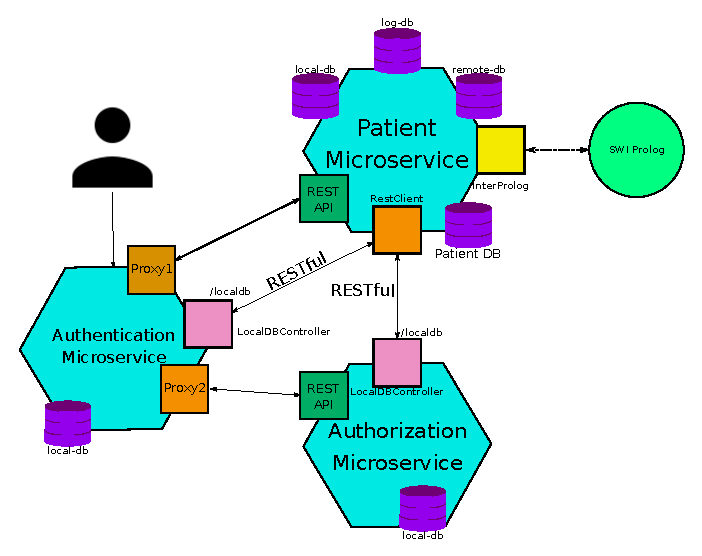
\includegraphics[width=\textwidth]{./figs/mrs-mics-target2.eps}}
            \caption[]%
            {{\small $\demo$ instrumented by $\tool$ using version 2 in Figure \ref{fig:brk-horn}.}}    
            \label{fig:mrs-mics-target2}
        \end{subfigure}
        \vspace{5mm}
        \caption[]
        {\small Architecture of microservices after instrumentation.} 
       \label{fig:mrs-structure}
    \end{figure*}

%\begin{figure} 
%	\centering
%	\fbox{\includegraphics[width=0.45\textwidth]{./figs/mrs-mics-target.eps}}
%	\caption{High-level architecture of $\demo$ after instrumentation by $\tool$ using version 1 and 3 specifications of Figure \ref{fig:brk-horn}.}
%	\label{fig:mrs-mics-target}
%\end{figure}
%
%\begin{figure} 
%	\centering
%	\fbox{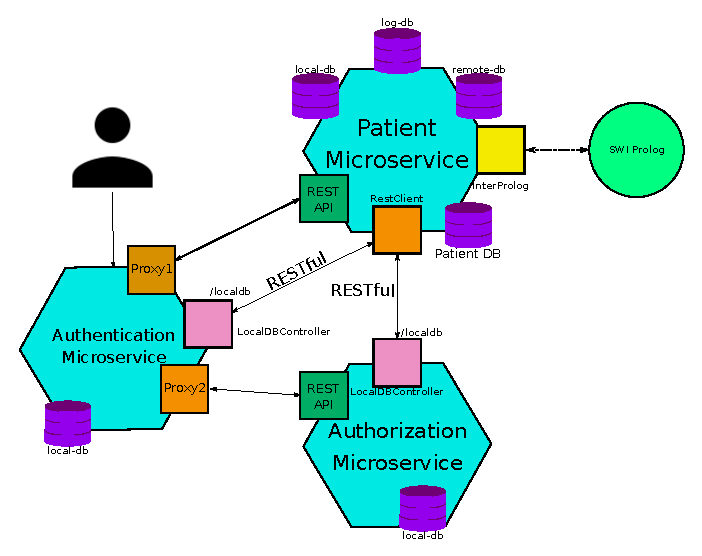
\includegraphics[width=0.45\textwidth]{./figs/mrs-mics-target2.eps}}
%	\caption{High-level architecture of $\demo$ after instrumentation by $\tool$ using version 2 specification of Figure \ref{fig:brk-horn}.}
%	\label{fig:mrs-mics-target2}
%\end{figure}

